\documentclass[../poma-notes.tex]{subfiles}

\begin{document}

\subsection*{Mean Value Theorems}

\begin{definition}
  Let $f$ be a real function defined on a metric space $X$. We say that $f$ has a \textit{local maximum} at a
  point $p \in X$ if there exists $\delta > 0$ such that $f(q) \le f(p)$ for all $q \in X$ with $d(p,q)<\delta$.
\end{definition}

\begin{anote}
  设 $f$ 是定义在度量空间 $X$ 上的实函数,那么 $f$ 在点 $p \in X$ 有 \textbf{局部极大值},如果存在 $\delta > 0$,对任意
  $q \in X$ 且 $d(p,q) < \delta$ 有 $f(q) \le f(p)$。局部极小值的定义类似。
\end{anote}

下一个 Theorem 是很多微分应用的基础。

\begin{theorem}
  Let $f$ be defined on $[a, b]$; if $f$ has a local maximum at a point $x \in (a, b)$, and if $f'(x)$ exists,
  then $f'(x) = 0$.
\end{theorem}

\begin{proof}
  根据 Definition 5.7 选取 $\delta$,使得
  \[
    a < x - \delta < x < x + \delta < b
  \]
  如果 $x - \delta < t < x$,那么
  \[
    \frac{f(t) - f(x)}{t - x} \ge 0
  \]
  令 $t \to x$,可知 $f'(x) \ge 0$。

  如果 $x < t < x + \delta$,那么
  \[
    \frac{f(t) - f(x)}{t - x} \le 0
  \]
  可知 $f'(x) \le 0$。因此 $f'(x) = 0$。
\end{proof}

类似的论证对于局部极小值同样成立。

\begin{anote}
  设 $f$ 定义在 $[a, b]$ 上;$x \in [a, b]$,如果 $f$ 在点 $x$ 取得局部极大值而且 $f'(x)$ 存在,那么 $f'(x) = 0$。
\end{anote}

\begin{theorem}
  If $f$ and $g$ are continuous real functions on $[a, b]$ which are differentiable in $(a, b)$, then there is
  a point $x \in (a,b)$ at which
  \[
    [f(b) - f(a)] g'(x) = [g(b) - g(a)] f'(x).
  \]
\end{theorem}

注意两个端点无需具备可导性。

\begin{proof}
  令
  \[
    h(t) = [f(b) - f(a)] g(x) = [g(b) - g(a)] f(x) \qquad (a \le t \le b)
  \]
  那么 $h$ 则在 $[a, b]$ 上连续,$h$ 在 $(a, b)$ 上可导,且
  \begin{equation}
    h(a) = f(b) g(a) - f(a) g(b) = h(b)
  \end{equation}
  为了证明该定理,我们需要得出对于某些 $x \in (a,b)$ 有 $f'(x) = 0$。

  如果 $h$ 是常数,那么对于所有 $x \in (a, b)$ 成立。如果对于某些 $t \in (a, b)$ 有 $h(t) > h(a)$,令 $x$ 为 $[a,b]$ 上的
  一点,其中 $h$ 达到其最大值(Theorem 4.16)。根据 (12),$x \in (a, b)$,以及 Theorem 5.8 可知 $h'(x) = 0$。如果对于某些
  $t \in (a, b)$ 有 $h(t) < h(a)$,那么该论点在选取 $[a, b]$ 中点 $x$,且 $h$ 达到其最小值时,同样成立。
\end{proof}

\begin{anote}
  已知:
  \begin{align*}
    \begin{cases}
      f'(x) = \frac{f(b) - f(a)}{b - a} \\
      g'(x) = \frac{g(b) - g(a)}{b - a}
    \end{cases}
  \end{align*}
  相除可得:
  \begin{align*}
    \begin{split}
      \frac{f'(x)}{g'(x)} & = \frac{f(b) - f(a)}{g(b) - g(a)} \\
      [f(b) - f(a)] g'(x) & = [g(b) - g(a)] f'(x)
    \end{split}
  \end{align*}
\end{anote}

该定理通常被称为 \textit{泛化中值定理};接下来的特殊例子则被称为 \say{真} 中值定理:

\begin{theorem}
  If $f$ is a real continuous function on $[a, b]$ which is differentiable in $(a, b)$, then there is a point
  $x \in (a, b)$ at which
  \[
    f(b) - f(a) = (b - a) f'(x)
  \]
\end{theorem}

\begin{proof}
  在 Theorem 5.9 中,取 $g(x) = x$。
\end{proof}

\begin{figure}[h]
  \centering
  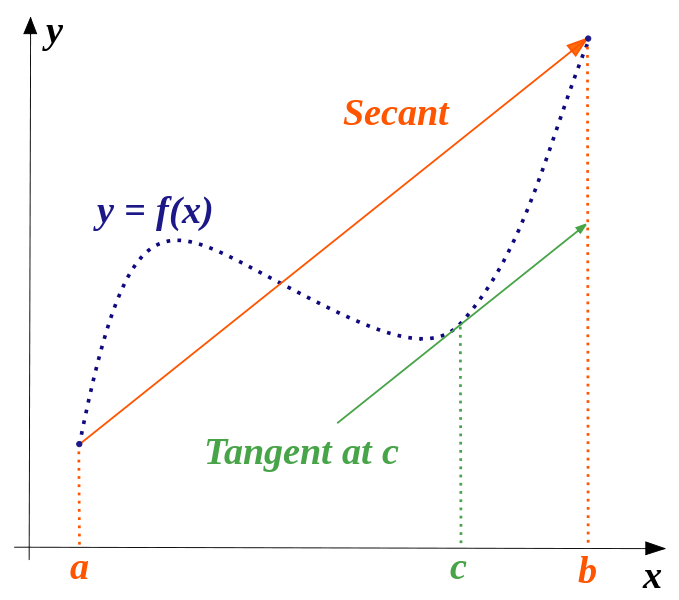
\includegraphics[width=0.5\textwidth]{\subfix{../images/mean-value-theorem.png}}\par
  \textbf{一般中值定理}:设 $f$ 是定义在 $[a, b]$ 的连续实函数,在 $(a, b)$ 内可导,那么一定有一点 $x \in (a, b)$,使得
  $f(b) - f(a) = (b - a) f'(x)$。
\end{figure}

\begin{theorem}
  Suppose $f$ is differentiable in $(a, b)$.
  \begin{enumerate}[label=(\alph*)]
    \item If $f'(x) \ge 0$ for all $x \in (a,b)$, then $f$ is monotonically increasing.
    \item If $f'(x) = 0$ for all $x \in (a,b)$, then $f$ is constant.
    \item If $f'(x) \le 0$ for all $x \in (a, b)$, then $f$ is monotonically decreasing.
  \end{enumerate}
\end{theorem}

\begin{proof}
  所有的结论都可以从该等式得出
  \[
    f(x_2) - f(x_1) = (x_2 - x_1) f'(x)
  \]
  其中 $x_1, x_2 \text{ in } (a, b)$。
\end{proof}

\end{document}
